\documentclass[twocolumn]{article} % Otras clases como report o book también pueden funcionar.

\usepackage[utf8]{inputenc} % Para usar caracteres UTF-8
\usepackage{lipsum} % Para generar texto de ejemplo
\usepackage{titlesec}
\usepackage{float}
\usepackage{tikz}
\usetikzlibrary{shapes, arrows.meta}

% Cambiar el tamaño de los títulos de sección a \normalsize
\titleformat{\section}{\normalsize\bfseries}{\thesection}{1em}{}
\titleformat{\subsection}[hang]{\small\bfseries}{\thesubsection}{1em}{}

\begin{document}

\title{Design, implementation and testing of a blockchain to avoid fraud on second hand vehicle sales}
\author{Julio Álvarez Villaescusa}
\date{\today}
\maketitle

\twocolumn[
    \begin{@twocolumnfalse}
        \begin{abstract}
            Blockchain technology has emerged as a revolutionary framework for secure, decentralized record-keeping, offering promising applications across various industries. Blockchain has plenty of room to explore new applications, and in this thesis we will explore the usage of blockchain to avoid fraud on second-hand car sales.
        \end{abstract}
        \vspace{1cm} % Espacio opcional para separar el abstract del resto del texto 
    \end{@twocolumnfalse}
]

\section{Fraud on second hand cars}
Fraud on second-hand car sales is a huge topic around the world, second hand cars can be a blessing, since they give access to vehicles to people who can't afford or don't want to pay for a brand new car, but they also can turn into a real nightmare. Malfunctioning cars can be sold disguised as normal second-hand cars with a slight temporary repair, which will end up in insanely expensive repairs for the person who got scammed.

On a daily basis, many cars are sold with issues that only the seller knows and only experts could notice. How can be prevent this scams with current technologies?

\section{Blockchain fundamentals}
Blockchain technologies have been popping up since the increase of the price of crypto-coins, and they have been in people's mouths ever since, but, are blockchain's only use to hold and distribute crypto-coins?

\subsection{Properties of a blockchain}
Blockchain is a decentralized digital ledger that securely records transactions across multiple computers in a way that makes it nearly impossible to alter the information.\\

\textbf{Structure:} Blockchain consists of a series of blocks, each containing a list of transactions. Each block is linked to the previous one through a unique identifier called a cryptographic hash, forming a chain like the one in Figure \ref{fig:simple_blockchain}.\\

\textbf{Transactions:} When a transaction is initiated, it is broadcast to a network of computers, or "nodes". These nodes verify the transaction's validity based on predefined rules (e.g., checking if the sender has enough balance).\\

\textbf{Consensus Mechanism:} Before adding a transaction to the blockchain, the network must agree that the transaction is valid. This consensus is typically achieved through mechanisms like Proof of Work (PoW) or Proof of Stake (PoS), ensuring that only valid transactions are added to the chain.\\

\textbf{Block Creation:} Verified transactions are grouped into a block. In PoW systems, miners compete to solve a complex mathematical problem; the first to solve it gets to add the block to the blockchain and is rewarded.\\

\textbf{Immutability:} Once added to the blockchain, the information of a block cannot be altered without changing all subsequent blocks, which requires majority control of the network. This makes the blockchain highly secure and tamper-resistant.\\

\textbf{Decentralization:} Unlike traditional ledgers controlled by a central authority, the blockchain is distributed across all nodes in the network, making it more resilient to attacks and ensuring transparency.\\

\begin{figure*}[h]
    \centering
    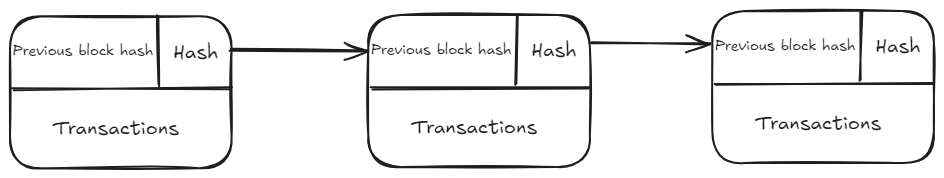
\includegraphics[width=1\textwidth]{Images/Simple_blockchain.png} 
    \caption{Simple blockchain.}
    \label{fig:simple_blockchain}
\end{figure*}
\newpage
\section{Vehicles and blockchain}
After taking a look at the blockchain's properties, we can see that some of the properties can be helpful on the fight to stop car fraud, but how do we implement a blockchain that is robust and safe at the same time that it does that job?\\

\noindent \textbf{We will need two extremely important things:}

\subsection{Transactions}
We will have various transactions or events that will be reflected on the blockchain.\newline

\textbf{Car transactions:} When a car is transferred, it will be reflected on the blockchain, indicating the key of the person who bought it, the person who sold it, the verifier of the transaction and, of course, the NFT of the car.\newline

\textbf{Accidents:} When a car gets in an accident, it will be reflected on the blockchain, where the NFT of the car will be indicated, as well as the driver's key, along with the severity of the accident and the verifier's key.\newline

\textbf{Vehicle inspections (ITV):} When a vehicle undergoes an inspection, the status of the car will be reflected on the blockchain, especially the kilometers performed on the vehicle. \newline  





\subsection{Actors}
To implement the blockchain, we will need nodes that satisfy different properties.

\textbf{General users:} They are owners, or past owners of vehicles. They don't have direct access to post on the blockchain, but they are able to consult it. They are represented as a key on the blockchain. \newline


\textbf{Insurance companies:} They are in charge of reflecting accidents on the blockchain, they are the verifiers of the accident transactions.\newline

\textbf{Public organs:} They are public organizations responsible for vehicle regulation such as the DGT. They are responsible for posting on the blockchain car transfers and are the verifiers of them.\newline

\textbf{Vehicle inspection services:} They are responsible for reflecting vehicle inspections on the blockchain.\newline

\textbf{Car manufacturers:} They will be in charge of posting the first reference to the car on the blockchain.



\subsection{Actors and transactions summary}

\begin{tabular}{|c|c|}
    \hline
    \textbf{Actors} & \textbf{Transactions} \\
    \hline
    Insurance companies & Accident transactions  \\
    \hline
    Public organs & Car transactions \\
    \hline
    Vehicle inspection services & Vehicle inspections \\
    \hline
    General users & - \\
    \hline
    
\end{tabular}

\newpage
\subsection{Avoiding fraud on vehicle sales}
After looking at transactions and actors, we can conclude that we can create a system that will help us avoid fraud. \newline

\noindent Let us take as an example a person who is trying to find a second hand car to buy, as the current vehicle's market prices are over the roof. When trying to find the best option, he may encounter offers that promise cars that only had one previous owner, which usually comes with an "it was driven by an old person and it has never gone through an accident".\newline

\noindent Without the blockchain, that person will have to decide whether to trust the stranger's words or not, and will be extremely hard, or even sometimes impossible to check if the conditions indicated by the seller are real or not.\newline

\noindent With the blockchain, that person will only need to ask for the seller's car NFT, and check the history of that car in the blockchain to decide if the deal is a good option or not.\newline


\section{How does our blockchain work?}

Every node will be connected to other nodes on the blockchain, accepting only connections from nodes that are allowed and verified to participate on the blockchain. When a node wants to post a transaction on the blockchain, it will broadcast it to the network. \newline

\noindent When enough transactions are received, a node will post the block after checking all transactions by broadcasting the block to the network.

\subsection{Receiving transactions}
After receiving a transactions a node will have to check if the node that sent the transaction is allowed to send transactions on the blockchain, if it is and the transaction is not already stored, the node will store it, otherwise it will be discarded.

\noindent If I am the node in charge of posting the block, after accepting a transaction, I will have to check if I got enough transactions to post the block, if I do, then I will do it. This behavior can be seen in Figure~\ref{fig:transactions_diagram}.
\newline

\begin{figure}[h] % [h] indica que queremos que esté en la posición aproximada de su inserción
    \centering
    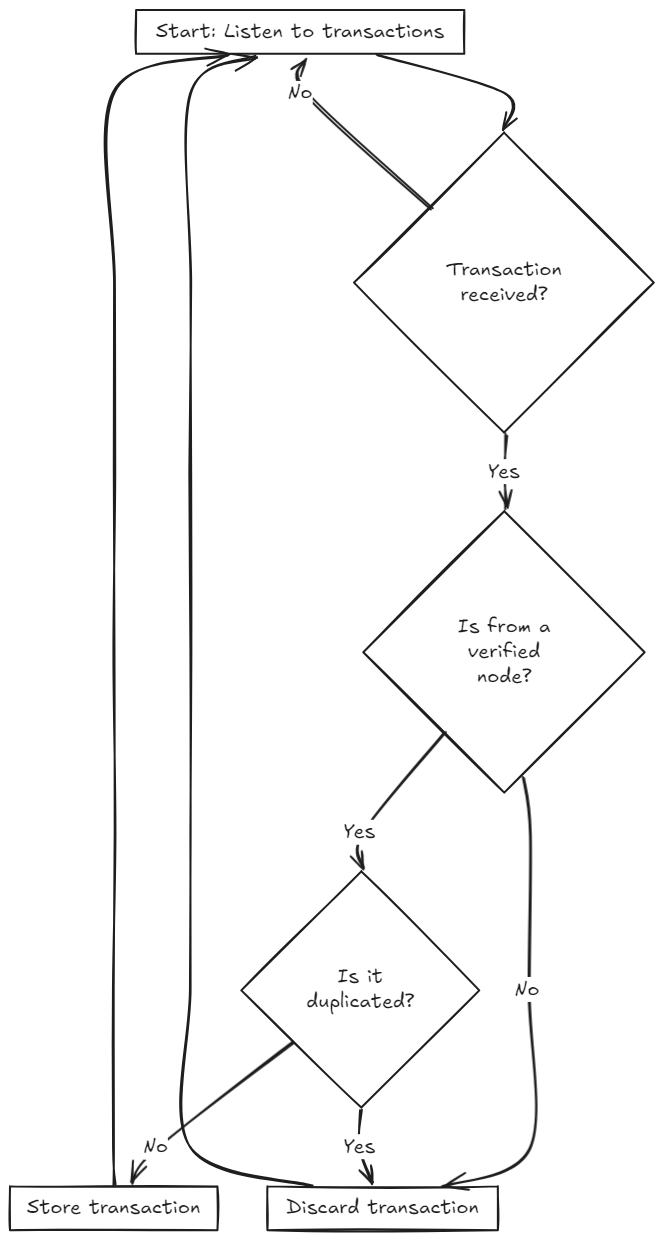
\includegraphics[width=0.94\columnwidth]{Images/transactions_diagramV2.png}
    \caption{Transaction flowchart} 
    \label{fig:transactions_diagram}
\end{figure}
\newpage

\subsection{Receiving blocks}
When a node receives a block, it will have to check if the block comes from the node that is in charge of posting the block, if the block has its corresponding hash, and if the transactions are the same as those he has stored previously. This behavior can be seen in Figure~\ref{fig:block_receival_diagram}.

\begin{figure}[h] % [h] indica que queremos que esté en la posición aproximada de su inserción
    \centering
    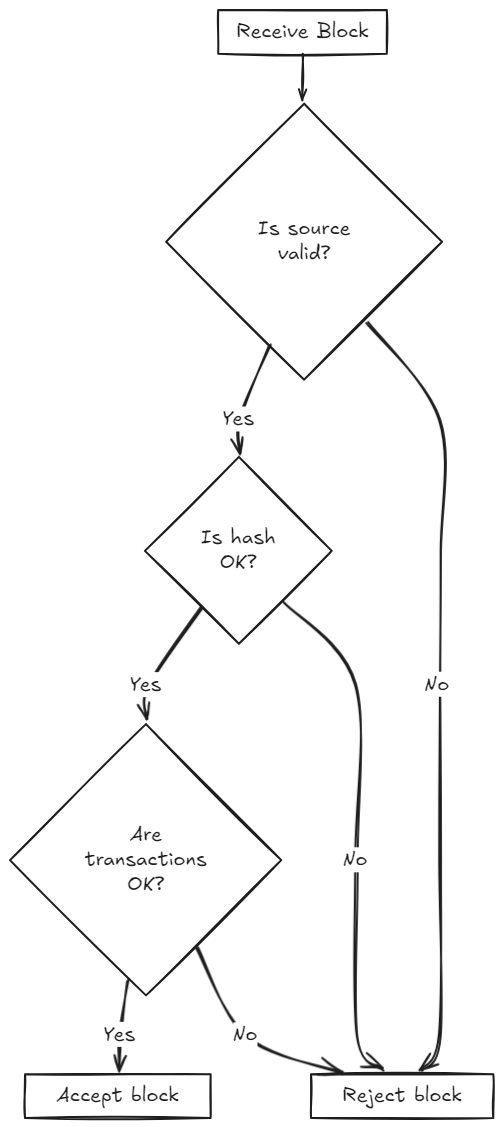
\includegraphics[width=0.9\columnwidth]{Images/block_receival_diagram.png}
    \caption{Block receival flowchart} 
    \label{fig:block_receival_diagram}
\end{figure}

\section{Implementation \& testing}
To implement this blockchain, I will use Python as the programming language and MongoDB to store the information locally on each node.\newline

\noindent For the testing part I will use Docker, where, each container will simulate a node and will interact with other containers.
\section{Conclusions}
What is the point of using a distributed ledger instead of a normal database?

\begin{itemize}
    \item \textbf{More security:} Distributing the information through different systems makes it harder to hack and nearly impossible to modify, since many devices constantly check the network.
    \item \textbf{More transparency:} Making it easier to track improper usage and easier to find the culprits.
    \item \textbf{Less intermediating costs:} Since the blockchain checks are automated, there is no need for intermediators to constantly check the blockchain manually.
    \item \textbf{Less bureaucracy involved:} The blockchain makes communications more simple and secure, therefore there will be less bureaucracy involved, which means faster processes. 
\end{itemize}
\end{document}